\documentclass[12pt]{article}
\usepackage{graphicx} % Required for inserting images
\usepackage{float}   

\usepackage[left=2.5cm,right=2.5cm, top =2.5cm, bottom = 2.5cm]{geometry}

\title{EC338 Assignment 2 - Group T}
\author{Aarush Bathula (5513578), Edward Chamberlain (5526786), \\
Jamie Chan (5534070), Will Murphy (2204888)}
\date{16 December 2025}

\begin{document}

\maketitle

\section{Descriptive Analysis}

\textit{Q: A policy maker is interested in finding out the impact of gender quotas on the share of female councillors. They have done some descriptive analysis of the data, and they observe that in 2011 elections, the share of female councillors is around 40\% in municipalities with quotas, compared to close to 30\% in municipalities without quotas.  Discuss briefly whether it would be appropriate to interpret the difference between these numbers as the causal impact of
quotas.} \\

\textbf{No.} We cannot claim the difference is the causal impact of quotas, as it is purely descriptive and cross-sectionally compares municipalities that might differ in other ways at a single point. Municipalities with populations above 3000 may systematically differ (more urban or different cultural preferences) in pre-quota female representation. The 10 pp. difference combines both the causal impact and pre-quota selection bias. Without counterfactuals such as parallel trends, or quasi-random assignment, we cannot state a causal impact. There might also be potential SUTVA violations.

\section{Difference-in-Differences}

\textit{a. Using a difference-in-differences strategy, estimate the impact of the quota on the share of female councillors.} \\

Using a 2x2 DiD  we estimate the ATET of the 2011 gender quota. The treated group is municipalities with over 3000 inhabitants in 2011, the control group are municipalities with under 3000 inhabitants. The pre period is the 2007 local election, as this is the final year before the quota was extended, and the post period is the 2011 election. We cluster standard errors at the municipality level as this is the level treatment is assigned . Our results, shown in \textbf{Table 1}, find the quota increases the share of elected female councillors by 6.3 percentage points.\\

As a robustness check, we estimated the DiD using within-municipality fixed-effects, showing a smaller 4.0 percentage point increase in the share of female councillors from the quota. Both results are significant at the 1\% level. \\
\begin{table}[H]
    \centering
    \caption{DiD estimates of quota effect on share of female councillors (2011)}
    \resizebox{\textwidth}{!}{%
    \begin{tabular}{lcccccc}
        \hline\hline
        & DiD Coefficient & Std. error & t & p-value & 95\% CI\\
        \hline
        Main estimate (2011) 
        & 0.063 & 0.006 & 10.90 & 0.000 & [0.052;\, 0.074] \\
        Fixed Effects Model 
        & 0.040 & 0.005 & 7.31 & 0.000 & [0.029;\, 0.051] \\
        \hline\hline
    \end{tabular}%
    }
\end{table}

\noindent
\textit{b. Under which assumptions does your DID analysis provide a consistent estimate of the Average Treatment Effect on the Treated (ATET)? Discuss whether they are likely to hold in this context. Provide some hypothetical example of why these assumptions might not hold.} \\


The DID estimator requires the parallel trends assumption, absent  the treatment, treated and control municipalities would follow the same trajectory, to hold. The event study, as seen in \textbf{Figure 1}, provides strong support for parallel trends: pre-treatment coefficients for 1999 ($-0.008$, $p=0.298$) and 2003 ($-0.005$, $p=0.356)$ are statistically insignificant and economically small, indicating no differential trends before the 2011 quota. The 2011 coefficient ($0.037$, $p<0.001$) confirms a positive treatment effect. \\

However, parallel trends could be violated if treated municipalities ($\geq$ 3000 population) were implementing complementary gender policies pre-2011, or if migration patterns systematically changed female political participation differently across groups. SUTVA may fail if the adoption of quota in neighboring municipalities generates spillovers through regional party strategies.

\section{Regression Discontinuity Design}

\textit{a. Now estimate the impact of the quota on the share of female councillors using a RDD empirical strategy and data for the 2011 elections. Provide (i) a RD plot and (ii) a table with your estimates. }\\

 Using a sharp RDD, at the 3000 population cutoff, we estimate the effect of quotas on the share of female councillors. The RD plot, \textbf{Figure 2}, shows a clear visual discontinuity at the cutoff, illustrating the policy's effect. Using the rdrobust local linear estimator, triangular kernel and the mean squared error optimal bandwidth(h=1111.475), we obtain an estimate that the share of females being elected was 4.4\% points higher for municipalities which received quotas. Our results are shown in \textbf{Table 2}. The result was significant at the 5\% significance level however we failed to reject the result at the 1\% significant level (p=0.022). In conclusion, the result displays a moderate causal effect of quotas on female representation in elected parties.

\begin{table}[H]
    \centering
    \caption{RDD estimates of quota effect on share of female councillors (2011)}
    \resizebox{\textwidth}{!}{%
    \begin{tabular}{lcccccc}
        \hline\hline
        & RD effect & Std. error & z-stat & p-value & 95\% CI & Bandwidth (L/R) \\
        \hline
        Main estimate (2011) 
        & 0.044 & 0.019 & 2.29 & 0.022 & [0.006;\, 0.082] & 1111.5 / 1111.5 \\
        Placebo (2007 outcome) 
        & 0.010 & 0.017 & 0.55 & 0.583 & [-0.037;\, 0.066] & 902.0 / 902.0 \\
        \hline\hline
    \end{tabular}%
    }
\end{table}

\noindent
\textit{b. Under which assumptions is the RDD analysis valid? Provide supporting evidence.} \\

To validate RDD, we must assume that municipalities can’t manipulate the population to sort around the threshold to obtain or avoid the quota. A density test displayed in figure 3 highlights that no significant manipulation occurs.\\

We must also assume that the relationship between the population and outcome (share of female councillors) evolves smoothly around the cutoff prior to the treatment. A placebo RDD test using the pre-treatment 2007 election results showed no discontinuity at the cutoff (Figure 4, p=0.583, RD effect = 0.010). \\

Finally, we must assume no other policies were implemented simultaneously during the quota treatment, that coincide with the 3000 population cutoff. Overall, the placebo and density tests provide enough evidence supporting the continuity assumption and validity of RDD.\\

\noindent
\textit{c. DID vs RDD: Discuss the difference between DID and RDD in terms of the plausibility of the underlying assumptions in this context, their precision, and the corresponding target estimand.}\\

In this context, RDD is more credible than DID. Although our events study in 2b demonstrates the parallel trends assumption holds, this could fail to hold if smaller municipalities are different to larger ones in ways that matter for politics such as candidate availability or voter attitudes, providing a poor counterfactual (Bagues and Campa, 2020). In contrast, RDD exploits quasi-random assignment around the population threshold of the quota exposure. By restricting the bandwidth, RDD provides a more plausible comparison between the treated and control groups supported by our validation tests in 3b.\\

However RDD is less precise due to the reduced sample size. In addition, the estimands differ, DID yields the Average Treatment Effect for treated municipalities (ATET) whereas RDD presents the Local Average Treatment Effect (LATE) for municipalities near the cutoff.\\

\section{Instrumental Variables Analysis}

\textit{a. First try to answer this question using a simple identification based on observables strategy (i.e., regress femalemayor on the share of female councillors, with some controls). Discuss whether this estimate might be interpreted causally.}\\

A 1\% point increase in the share of females increases the probability of a female being a mayor by 0.64\% points, with the result being significant (p=0.000). However, this estimate cannot be interpreted causally due to endogeneity. The estimate is likely upward biased due to omitted variable bias (municipalities with progressive political attitudes drive both outcomes) and reverse causality (female mayors incentivise parties to increase female representation).As a result, the OLS estimate captures correlation, not causation.\\

\noindent
\textit{bi. Let us now address this question combining a DID identification with an instrumental variables strategy, where we use quotas as an instrument for the share of female councillors:
i. Discuss whether the instrument is relevant.(Hint: check your previous DID in 2a.)} \\

Our first stage regression reveals that after the 2011 political reforms, treated municipalities elected 4.08\% point more female councillors compared to non-treated ones, with the results being statistically strong and significant (p=0.000). Furthermore, given we obtained an F statistic of 56.5 (from testparm on the instrument), we can conclude that the instrument satisfies the relevance condition (F$>$10) under a year fixed effects model.\\

\noindent
\textit{ii. Estimate the reduced form regression. (Hint: run your DID using now as the outcome variable whether a woman is elected mayor.)}\\ 

Our reduced form regression implies that the 2011 quota reforms of females has an insignificant result of the probability of electing a female mayor (p=0.405), indicating that the quota did not have a detectable average effect on the likelihood of electing a female mayor. This result does not reject a zero effect but is consistent with either a small true effect or limited statistical power.\\

\noindent
\textit{iii.  Wald estimate: Based on the first stage coefficient from 2a and the reduced form coefficient from (ii), calculate the IV estimate of the impact of women in the council on the probability that a woman is 
elected mayor. (Hint: Divide manually the reduced form by the first 
stage.)} \\

Our Wald IV Estimate yields a coefficient of 0.35, obtained by dividing the reduced form coefficient by the first stage effect. This implies that a one percentage point increase in the share of female councillors increases the probability of a female being elected by 0.35\% points. However, this result should be interpreted cautiously, given the insignificance of the reduced form coefficient.\\

\noindent
\textit{c. Calculate the IV estimate using 2SLS. Is it similar to the one you found in (b.iii)? Now you also have standard errors. Is the estimate statistically significant? In terms of magnitudes, what is the largest effect that you can reject?}\\

Using 2SLS, the IV estimate implies that a 1 percentage point increase in the share of female councillors increases the probability of a female becoming a mayor by 0.35 percentage points with a robust standard error of 0.42. The estimate is identical in magnitude and sign to the Wald estimate found in b)iii. The estimate is statistically insignificant (p=0.405), therefore we fail to reject that the null hypothesis is zero. Based on the 95\% confidence interval, we can reject estimates outside the range (-0.475, 1.177), implying that only relative large effects can be rejected.\\

\noindent
\textit{d. Discuss whether, in this context, the IV assumptions are likely to hold. Hint: Discuss relevance, exogeneity and exclusion restriction.}\\

The relevance assumption holds: our first stage regression shows the quota reform significantly increased the share of female councillors. The exogeneity assumption is plausible, as quota assignment is as good as random conditional on municipality size and time, although cannot be directly tested. The exclusion restriction requires that the probability of females becoming a mayor holds only through the share of female councillors, not other political channels such as symbolic effects, which is unlikely. Monotonicity is likely to hold, requiring that no municipalities reduce their share of female councillors in response to the reforms. \\

\textit{Statement of Contribution}\\
\noindent
All members of the group contributed equally. \\

\clearpage

\section{Reference List}
\begin{itemize}
    \item Bagues M., Campa P. (2020). "Women and Power: Unpopular, Unwilling, or Held Back? A Comment"\textit{ Journal of Political Economy, University of Chicago Press}, vol.128(5), pp. 210-216.\\
\end{itemize}
\clearpage

\section{Appendix}
\begin{figure}[H]
    \centering \label{fig:event_study}
    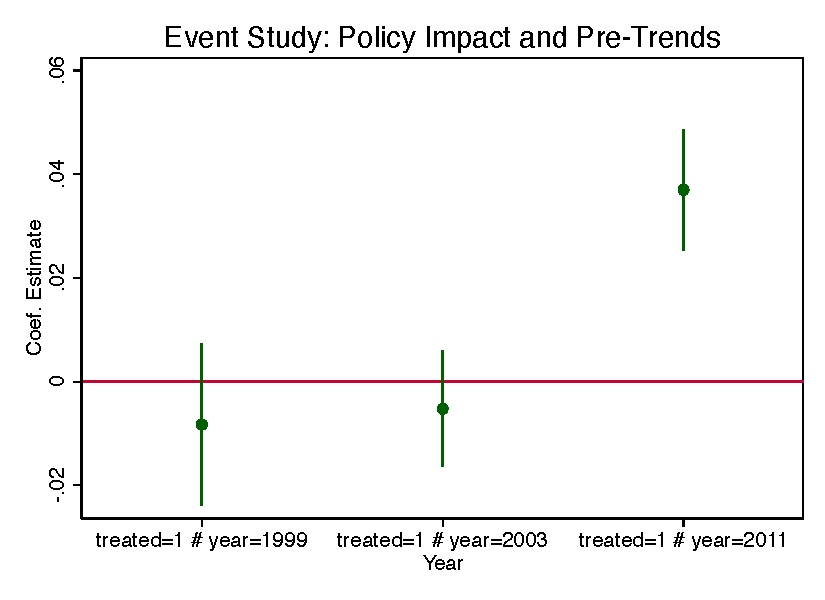
\includegraphics[width=0.8\textwidth]{q2_event_study_16dec}
    \caption{Event study: pre‑trends and policy impact}
\end{figure}

\begin{figure}[H]
    \centering
    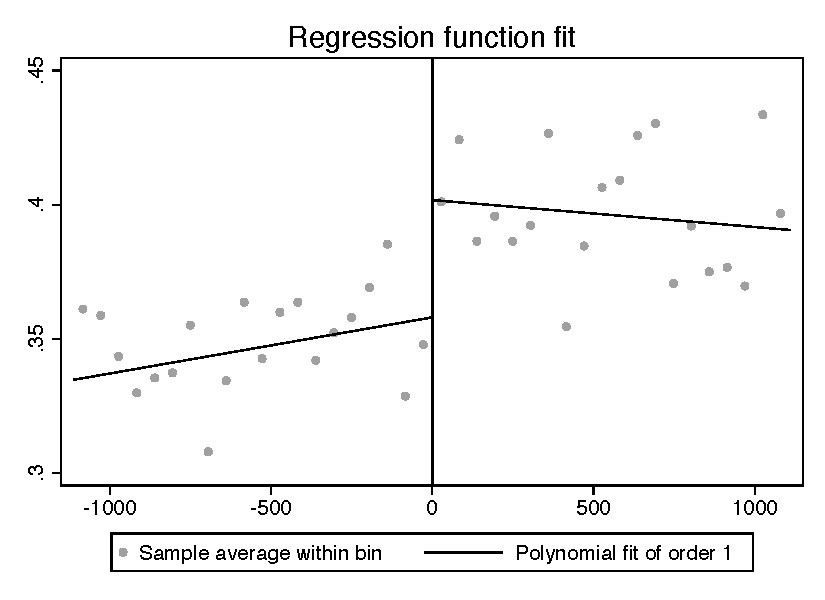
\includegraphics[width=0.8\textwidth]{rdplot_share_female_councillors_2011_16dec}
    \caption{RDD: Share of female councillors in 2011 around the 3,000 cutoff}
\end{figure}

\begin{figure}[H]
    \centering
    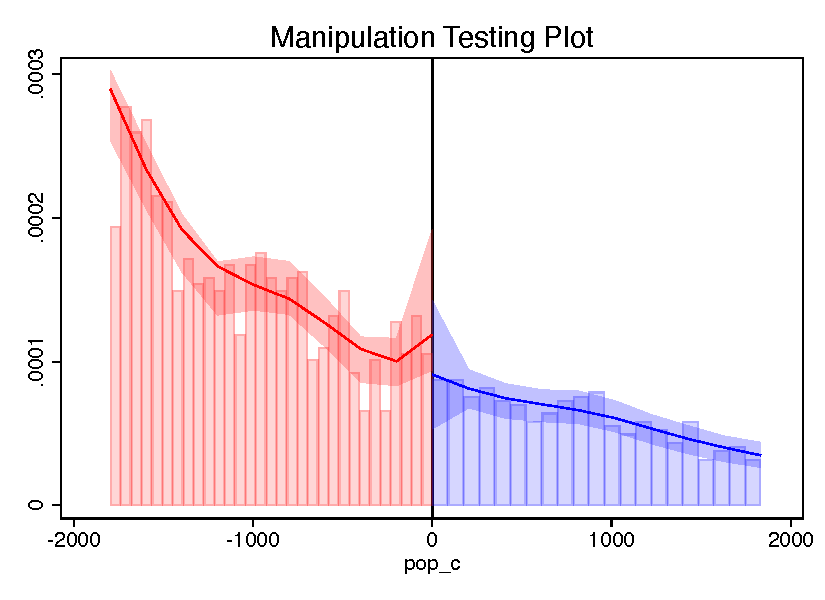
\includegraphics[width=0.8\textwidth]{rddensity_population_3000_16dec}
    \caption{Density of population around the 3,000 cutoff}
\end{figure}

\begin{figure}[H]
    \centering
    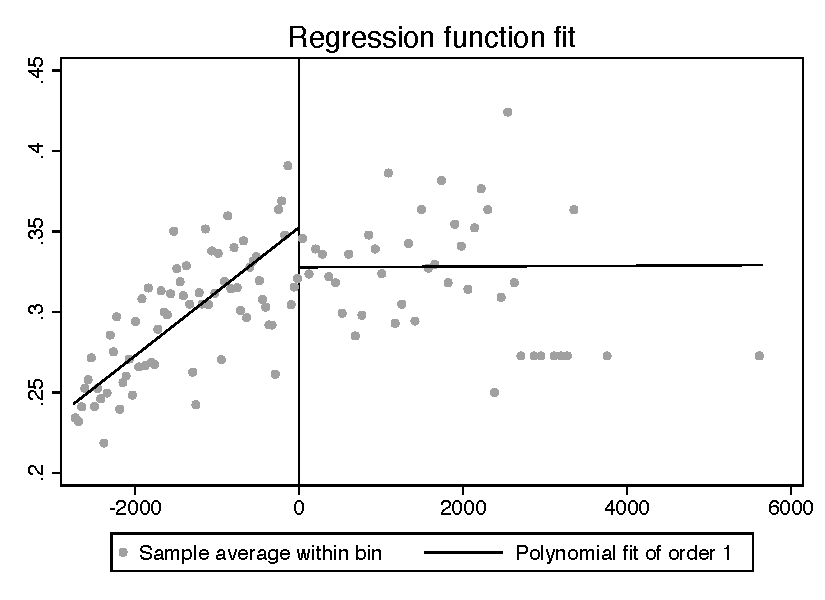
\includegraphics[width=0.8\textwidth]{rdplot_share_female_councillors_2007_placebo_16dec}
    \caption{Placebo RDD: Share of female councillors in 2007}
\end{figure}



\end{document}
